\documentclass[11pt]{article}
\usepackage[margin=1in]{geometry}
\usepackage[T1]{fontenc}
\usepackage[utf8]{inputenc}
\usepackage{lmodern}
\usepackage{amsmath,amssymb,amsthm}
\usepackage{booktabs}
\usepackage{tabularx}
\usepackage{enumitem}
\usepackage{xcolor}
\usepackage{listings}
\usepackage{tikz}
\usetikzlibrary{arrows.meta,positioning}
\usepackage[colorlinks=true,linkcolor=blue!50!black,citecolor=blue!50!black,urlcolor=blue!50!black]{hyperref}

\setlist{itemsep=2pt,topsep=4pt}
\emergencystretch=3em
\let\origus\_
\renewcommand{\_}{\origus\allowbreak}

\newtheorem{theorem}{Theorem}
\newcommand{\CP}{\mathbb{CP}^1}
\newcommand{\C}{\mathbb{C}}
\newcommand{\eps}{\varepsilon}
\newcommand{\code}[1]{\texttt{#1}}

% ---- Numbers from the axiom census (tests/ReportAxiomCensus.lean) ----
\newcommand{\NdeclClean}{1{,}194}
\newcommand{\NdeclSorry}{54}
\newcommand{\NthmClean}{748}
\newcommand{\NthmSorry}{48}

\lstdefinelanguage{lean}{
  morekeywords={theorem,lemma,def,structure,class,where,by,fun,let,have,exact,obtain,refine,sorry,import,namespace,end,variable,open},
  sensitive=true, morecomment=[l]{--}, morecomment=[s]{/-}{-/}, morestring=[b]"}
\lstset{language=lean,basicstyle=\ttfamily\footnotesize,keywordstyle=\bfseries\color{blue!50!black},
  commentstyle=\itshape\color{gray},columns=fullflexible,keepspaces=true,frame=single,framerule=0.3pt,
  xleftmargin=4pt,xrightmargin=4pt,breaklines=true,
  literate={→}{{$\to$}}1 {∀}{{$\forall$}}1 {∃}{{$\exists$}}1 {¬}{{$\neg$}}1 {≤}{{$\le$}}1 {ℕ}{{$\mathbb{N}$}}1
           {ℝ}{{$\mathbb{R}$}}1 {ℤ}{{$\mathbb{Z}$}}1 {⟨}{{$\langle$}}1 {⟩}{{$\rangle$}}1 {⌊}{{$\lfloor$}}1 {⌋}{{$\rfloor$}}1
           {σ}{{$\sigma$}}1 {∧}{{$\wedge$}}1 {∘}{{$\circ$}}1 {₁}{{$_1$}}1 {₂}{{$_2$}}1 {₃}{{$_3$}}1 {·}{{$\cdot$}}1}

\title{A Machine-Checked Architecture for Genus-Zero Gromov Compactness in Lean~4,\\
Built with Local Gemma Models and a Multi-Agent Harness}
\author{Pablo Su\'arez-Serrato}
\date{November 2026}

\begin{document}
\maketitle

\begin{abstract}
We report a Lean~4/Mathlib formalization project for Gromov's compactness theorem for genus-zero
pseudo-holomorphic curves in closed symplectic manifolds with tame almost-complex structure.
The development (32 modules, about 8{,}700 lines) states the theorem with concrete definitions:
energy as an integral of the energy density, $C^\infty_{\mathrm{loc}}$ convergence under moving
M\"obius frames, and stable sphere trees with nodal matching. It also contains a library of
machine-checked results using only Lean's standard axioms. These include three-point transitivity
and uniqueness for M\"obius maps, diagonal subsequence extraction, the combinatorial stability
bounds $G\le P-2$ and $|V|\le 2P-2$, the strict energy-rank decrease that drives the bubbling
induction, and a bridge from Mathlib's formalization of Hofer's lemma to the calibrated rescaling
step. The analytic core is \emph{not} yet formalized. It comprises $\eps$-regularity, elliptic
bootstrapping, cylinder decay, removal of singularities, and the existence statements of the
bubbling construction. It is stated precisely and left as 45 declarations containing
\code{sorry}. Consequently the master theorem currently depends on \code{sorryAx}. The work was
carried out in about 29 hours of wall-clock time by an agentic workflow in Google Antigravity.
Groups of 3--5 agents (implementers, reviewers, adversarial challengers and a forensic auditor)
worked in two stages per phase: interface scaffolding (``Model~A''), then proof completion
(``Model~B''). A locally served Gemma~2 (9B) model was available to the agents for tactic
suggestions. We describe the decomposition, the formal status, the workflow and its failure
modes, and the remaining work.
\end{abstract}

\section{Introduction}

Gromov's compactness theorem~\cite{Gromov85} is the foundation of the theory of
pseudo-holomorphic curves. Proofs with complete analytic detail are long; see
\cite{McDuffSalamon,Zinger,IvashkovichShevchishin}. To our knowledge no proof assistant
contains a formal proof. Mathlib~\cite{mathlib} has smooth manifolds, measure theory, and a
formalization of Hofer's lemma (\code{Mathlib.Analysis.Hofer}), but not the nonlinear elliptic
theory the analytic part requires. Symplectic geometry in Lean is being organized by the TauCeti
roadmap~\cite{TauCeti}.

This note records what was built, what is fully checked, and what remains. It also explains how
it was built. The project tested whether a consumer laptop running a local open-weights model
inside an agentic harness can produce a large, honest, reviewable formalization scaffold for a
research-level theorem in a few days. We claim a checked \emph{architecture} and a checked
\emph{combinatorial and algebraic layer}. We do not claim a complete formal proof of Gromov
compactness.

\paragraph{Target statement.}
Let $M$ be a compact boundaryless manifold with a closed nondegenerate two-form $\omega$ and an
almost-complex structure $J$ with $\omega(v,Jv)>0$ for $v\ne0$. Let
$g(v,w)=\tfrac12(\omega(v,Jw)+\omega(w,Jv))$ and let $E(u)=\tfrac12\int|du|_g^2$.

\begin{theorem}[Genus-zero Gromov compactness]\label{thm:main}
Let $u_n:\CP\to M$ be nonconstant $J$-holomorphic spheres with $E(u_n)\le B$. Then a subsequence
converges to a stable sphere tree $(T,\{u_v\},\{z_{vw}\})$. This means that there are M\"obius
frames $\phi_{v,n}$ such that $u_{\sigma(n)}\circ\phi_{v,n}\to u_v$ in $C^\infty_{\mathrm{loc}}$
away from the nodes of $v$, $\phi_{v,n}^{-1}\circ\phi_{w,n}\to z_{vw}$ locally uniformly away from
$z_{wv}$, and $E(u_{\sigma(n)})\to\sum_v E(u_v)$. Moreover, with $P$ principal and $G$ ghost
components and a fixed energy quantum $h>0$, one has $Ph\le B$, and for $|V|>1$ also $G\le P-2$,
$|V|\le 2P-2$.
\end{theorem}

\section{Mathematical source and decomposition}

The mathematical specification is a 17-page blueprint (\code{gromov\_compactness.pdf}, 3~November
2026). It writes the proof as 39 independently stated \emph{task contracts}. It follows the
standard route through Zinger's notes~\cite{Zinger}, using Lipyanskiy~\cite{Lipyanskiy} for the
concentration and bootstrapping arguments. It assumes no genericity, simplicity or rationality of
$[\omega]$. The contracts are grouped as follows.
\begin{itemize}
\item \textbf{F00--F06 (foundations):} library audit and toolchain pin; the target structure and
  Cauchy--Riemann equation; $\CP$ and the M\"obius group; the energy measure; $C^\infty_{\mathrm{loc}}$
  convergence; strictly monotone subsequences and diagonal extraction; labelled sphere trees.
\item \textbf{A01--A12 (local analysis):} mean-value inequality, Bochner inequality
  $\Delta e\ge -be^2$, $\eps$-regularity, interior $W^{k+1,p}$ estimates and Morrey embedding,
  nonlinear bootstrap, local compactness, the sphere energy gap $\eps_{\mathrm{sph}}>0$, target
  monotonicity, cylinder localization, exponential decay on long cylinders, extension across
  punctures, and removal of singularities.
\item \textbf{C01--C03, B01--B07 (concentration and bubbling):} weak compactness of energy
  measures; a finite singular set $S$ with $|S|\eps_{\mathrm{reg}}\le B$; the defect identity
  $\mu=\mu_{u_0}+\sum_{p\in S}m_p\delta_p$; a single threshold
  $0<h\le\min(\eps_{\mathrm{reg}}/2,\eps_{\mathrm{sph}},\eps_{\mathrm{neck}}/2)$; calibrated
  rescaling $E(f_n;D_{\lambda_n}(a_n))=m-h/2$; vanishing neck energy and diameter with explicit
  quantifier order; the one-level mass split $m=E(v)+\sum m_i$ with $f(0)=v(\infty)$; branching of
  constant bubbles; strict decrease of $\lfloor m/h\rfloor$; and well-founded induction producing a
  finite tree for each defect.
\item \textbf{G01--G05 (assembly):} global frames, stabilization of the root, the core theorem,
  component bounds, and an axiom audit.
\item \textbf{E01--E05 (extensions):} varying $J_n\to J$, marked points, homology class
  preservation, automorphism finiteness, and compactness and Hausdorffness of
  $\overline{\mathcal M}_{0,k}(M,J,\le B)$.
\end{itemize}
The blueprint fixes completion criteria (its \S4.3). A proof task is complete only if
\code{\#print axioms} reports no \code{sorryAx}. A conditional theorem must be labelled
conditional. It also lists eight stress cases for agents to check, including non-compact targets,
domain collapse $u_n(z)=nz$, ghost clusters, multiple covers, concentration on the calibration
circle, and colliding marked points. An implementation plan (\code{AUTOFORMALIZATION\_PLAN.md})
assigns each contract an owner file, acceptance tests and a role in the agent workflow. A
\code{leanblueprint} document (16 pages) tracks each contract's declaration and its
\verb|\leanok| status.

\section{The Lean development}

\paragraph{Setup.} Lean \code{v4.16.0}, Mathlib \code{v4.16.0}, built with \code{lake}. The
library has 32 modules and $\approx$8{,}700 lines, with 443 theorem/lemma declarations and 174
definitions, structures and instances. Adversarial test files (25 files, $\approx$7{,}400 lines)
written by challenger agents are kept under \code{tests/}. All modules build with no errors.

\paragraph{Definitions.} The target is a type class \code{ClosedTameTarget}. It carries pointwise
continuous bilinear forms $\omega_x$ with skew-symmetry and nondegeneracy, an endomorphism $J_x$
with $J^2=-1$, and the tameness inequality. $J$-holomorphicity is \code{ContMDiffOn} together with
$du\circ j=J\circ du$ via \code{mfderiv}. The energy measure is the push-forward from the
stereographic chart of Lebesgue measure with density $\tfrac12|du|_g^2$, and $E(u)$ is its real
total. A \code{StableSphereTreeLimit} contains a finite tree, component maps that are
$J$-holomorphic, nodal matching, and stability of constant components. Convergence is the
structure \code{CompactnessWitness}: a strictly monotone $\sigma$, frames $\phi_{v,n}$, and the
three conditions of Theorem~\ref{thm:main} as fields. \emph{Limitations:} the fields
\code{$\omega$\_closed} and \code{J\_smooth} are currently opaque \code{Prop}s, so closedness of $\omega$
and smoothness of $J$ are not yet expressed in terms of Mathlib's differential forms. More
seriously, the energy measure integrates the round-metric density against Lebesgue measure on
$\C$ without the conformal Jacobian of the chart. For a map with nonzero density at $\infty$ the
integral is infinite, and \code{toReal} then reports energy $0$. Until the definition is
corrected, several open statements, including the energy gap and the master theorem, are likely
false as stated. Correcting this definition is the first task of the completion plan.

\paragraph{Main statement.} The master theorem combines an existence theorem with the proved
component bounds:
\begin{lstlisting}
theorem gromov_compactness_genus_zero (th : Bubbling.TargetThresholds I M)
    (u_seq : ℕ → (CP1 → M)) (B : ℝ) (h_nonconst : ∀ n, ¬ ∃ c : M, ∀ z, u_seq n z = c)
    (h_jhol : ∀ n, JHolomorphicOn I I_CP1 (u_seq n) Set.univ)
    (h_energy : ∀ n, totalEnergy I (u_seq n) ≤ B) :
    ∃ u_lim : StableSphereTreeLimit I, Nonempty (CompactnessWitness I u_seq u_lim) ∧
      (P * th.h ≤ B) ∧ (1 < |V| → G + 2 ≤ P ∧ |V| + 2 ≤ 2 * P) ∧ ((|V| : ℤ) ≤ max 1 (2 * ⌊B / th.h⌋ - 2))
\end{lstlisting}
(Here $P$, $G$, $|V|$ abbreviate the corresponding \code{Fintype.card} expressions.) The
existence part comes from \code{gromov\_compactness\_core}, whose proof is a single
\code{sorry}. The bounds part, \code{gromov\_compactness\_component\_bounds}, is fully checked.

\paragraph{What is fully checked.}
For every declaration of the library we computed the axioms it depends on
(\code{tests/ReportAxiomCensus.lean}). No project \code{axiom} is declared and no non-standard
axiom occurs. Counting all constants in the environment, including compiler-generated ones such as
structure projections and extensionality lemmas, \NdeclClean{} constants (\NthmClean{} theorems)
depend only on \code{propext}, \code{Classical.choice} and \code{Quot.sound}, and \NdeclSorry{}
constants (\NthmSorry{} theorems) depend on \code{sorryAx}.
Representative fully checked results:
\begin{itemize}
\item \emph{M\"obius geometry (F02).} Existence and uniqueness, up to scalars, of a M\"obius matrix
  sending one triple of distinct points of $\CP$ to another, proved with adjugate matrices. Also
  nontrivial affine dilations on the stereographic sphere. This is the longest module (1{,}314
  lines).
\item \emph{Metric and energy algebra (F01, F03).} Symmetry, positive-definiteness and
  $J$-invariance of $g$; $J$-holomorphicity is invariant under biholomorphic reparametrization;
  nonnegativity and monotonicity of the energy measure.
\item \emph{Bookkeeping (F05, F06).} Cantor diagonal extraction for nested strictly monotone
  subsequences; the degree sum $\sum_v\deg v=2(|V|-1)$ for sphere trees; the handshake argument
  giving $G\le P-2$.
\item \emph{Bubbling arithmetic (B01, B02, B04--B06).} A threshold $h$ exists once the analytic
  constants $\eps_{\mathrm{reg}},\eps_{\mathrm{sph}},\eps_{\mathrm{neck}}$ are supplied (a
  reduction; unconditional existence still depends on the open analysis). The Hofer
  doubling lemma from Mathlib is specialized to $(\C,|\cdot|)$ for gradient blow-up. Calibrated
  radii exist given the radial intermediate-value hypothesis. Child counts
  satisfy $|q|\le\lfloor m/h\rfloor$; a constant bubble has $\ge2$ children and degree $\ge3$, given
  the one-level decomposition; children satisfy $m_i\le m-h$; and
  $\lfloor m_i/h\rfloor<\lfloor m/h\rfloor$.
\item \emph{Measures (C01--C03).} Portmanteau-type consequences of weak convergence; finiteness and
  the cardinality bound $|S|\le\lfloor B/\eps_{\mathrm{reg}}\rfloor$ for the atom set; finite Dirac
  sums and total-mass identities.
\item \emph{Counting (G04, E02).} $Ph\le B$, $|V|+2\le2P$ and $|V|\le\max(1,2\lfloor B/h\rfloor-2)$;
  the marked versions with $k$ marked points; translation and scaling invariance of the
  cross-ratio.
\end{itemize}
Several of these are \emph{reduction theorems}: they are checked, but they take a statement from
the open layer as an explicit hypothesis. For example, ghost branching takes the one-level
decomposition as input. Such hypotheses appear in the theorem signatures.

\paragraph{What is open.}
There are 45 declarations with a direct \code{sorry}, grouped as follows.
(i)~\emph{Analysis (15):} mean-value inequality, Bochner inequality, $\eps$-regularity, interior
Cauchy--Riemann estimate, Morrey embedding, nonlinear bootstrap, local smooth compactness, energy
gap, target monotonicity, cylinder localization, cylinder decay, puncture extension, and removal
of singularities.
(ii)~\emph{Concentration and bubbling (14):} weak compactness of measures, existence of
concentration data, the defect identity, quantified neck vanishing, existence of the one-level
decomposition, resolution of a defect into a tree, global frame assembly, and stabilization.
(iii)~\emph{Core (2):} \code{gromov\_compactness\_core} and the constant/nonconstant alternative.
(iv)~\emph{Extensions (16):} varying-$J$ compactness, marked compactness, M\"obius rigidity for
automorphisms, stability $\Leftrightarrow$ finite automorphisms, and the moduli space. Here the
Gromov distance and the metric-space instance on $\overline{\mathcal M}_{0,k}$ are themselves
defined by \code{sorry}. The Hausdorff property \code{moduli\_space\_t2} is derived from that
instance and therefore has no mathematical content yet.
Group~(i) is the main obstacle: Mathlib lacks the $L^p$ theory of the Cauchy--Riemann operator and
the needed geometric measure theory. These are substantial library projects in their own right.

\section{Workflow: Antigravity, Gemma and 3--5 agents}

\paragraph{Harness.} The work ran in Google Antigravity, an agentic development environment.
Agents in Antigravity can read and edit files, run shell commands (\code{lake build}, LaTeX, git)
and start other agents. A top-level ``teamwork'' agent received the user's instructions and
delegated them to per-phase orchestrators. Orchestrators started task agents, each with its own
working directory and a written hand-off report. The agents ran on a hosted Gemini model
configured in Antigravity.

\paragraph{Roles and concurrency.} At any moment the team typically had 3--5 active task agents:
\begin{itemize}
\item \textbf{Explorers} (usually three in parallel) surveyed Mathlib declarations and candidate
  proof strategies, sometimes querying the local Gemma model.
\item \textbf{Workers} (one per milestone) wrote the Lean code, ran \code{lake build}, and updated
  the blueprint.
\item \textbf{Verification gate} (five in parallel): two \emph{reviewers}, one for mathematical
  fidelity to the sources and one for type-class architecture and blueprint links; two
  \emph{challengers}, who wrote adversarial Lean test files for edge cases and stress cases; and a
  \emph{forensic auditor}, who looked for custom axioms, hidden \code{sorry} and premature
  \verb|\leanok|.
\item \textbf{Victory auditor}: one independent agent with no shared context. Before a phase was
  declared complete, it re-ran builds and tests and checked the git history.
\end{itemize}
Over the project, 222 agent working directories and 206 hand-off reports were created (37
explorer, 36 worker, 76 reviewer/challenger and 19 auditor directories, 15 orchestrators and 7
victory auditors).

\begin{figure}[t]
\centering
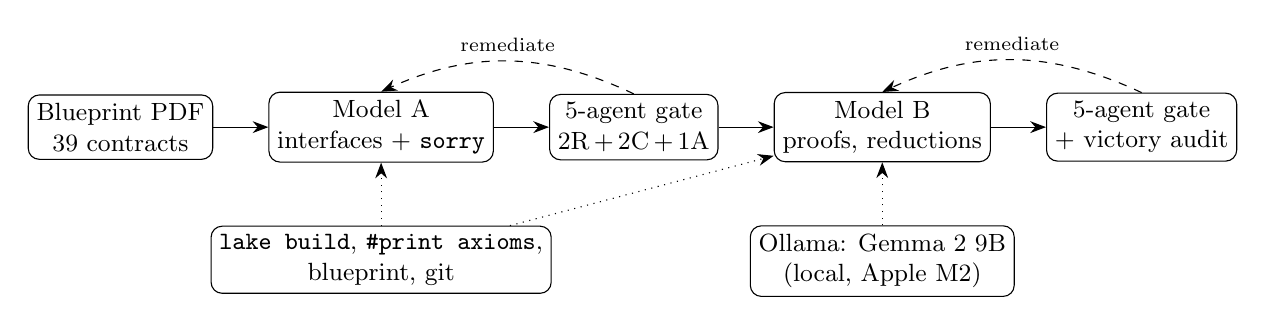
\begin{tikzpicture}[node distance=5mm and 7mm, every node/.style={font=\small},
  box/.style={draw,rounded corners,align=center,inner sep=3pt,minimum height=8mm},
  arr/.style={-{Stealth[length=2mm]}}]
\node[box] (spec) {Blueprint PDF\\39 contracts};
\node[box,right=of spec] (A) {Model A\\interfaces + \code{sorry}};
\node[box,right=of A] (gA) {5-agent gate\\2R\,+\,2C\,+\,1A};
\node[box,right=of gA] (B) {Model B\\proofs, reductions};
\node[box,right=of B] (gB) {5-agent gate\\+ victory audit};
\node[box,below=8mm of B] (oll) {Ollama: Gemma~2 9B\\(local, Apple M2)};
\node[box,below=8mm of A] (lean) {\code{lake build}, \code{\#print axioms},\\blueprint, git};
\draw[arr] (spec)--(A); \draw[arr] (A)--(gA); \draw[arr] (gA)--(B); \draw[arr] (B)--(gB);
\draw[arr,dashed] (gA.north) to[bend right=25] node[above,font=\scriptsize]{remediate} (A.north);
\draw[arr,dashed] (gB.north) to[bend right=25] node[above,font=\scriptsize]{remediate} (B.north);
\draw[arr,dotted] (oll)--(B); \draw[arr,dotted] (lean)--(A); \draw[arr,dotted] (lean)--(B);
\end{tikzpicture}
\caption{Per-phase workflow. R = reviewer, C = challenger, A = forensic auditor. Each phase was
committed to git and checkpointed after its gate.}
\label{fig:workflow}
\end{figure}

\paragraph{Two stages per phase.} The four phases were foundations (F00--F06); local analysis and
calibrated bubbling (A01--A12, B01--B02); iterative bubbling, tree induction and assembly
(C01--C03, B03--B07, G01--G05); and extensions (E01--E05). Each phase had two stages
(Fig.~\ref{fig:workflow}). \textbf{Model~A} wrote all definitions and theorem statements of the
phase with \code{sorry} proofs. These were required to typecheck and to be non-vacuous: no
\code{True} conclusions, no circular hypotheses, no \code{axiom}. This let later contracts compile
against fixed interfaces immediately. \textbf{Model~B} then replaced \code{sorry}s with proofs or
with checked reductions to clearly named open statements. Each stage ended with the five-agent
gate. A rejection sent the work back to the worker with the gate's findings. Each certified stage
was committed to git, and a JSON checkpoint was written by a small control script
(\code{tools/workflow\_control.py}). The script also implements \code{pause} and \code{resume}
through a sentinel file, and the user used it several times. Commits run from 3~November 07:49 to
4~November 12:34 (Pacific time).

\paragraph{Local compute with Gemma.} To limit hosted-model usage, a stdlib-only Python client
(\code{tools/}\allowbreak\code{ollama\_lean4\_client.py}) exposes \code{health}, \code{autoformalize},
\code{suggest-tactic} and \code{repair} commands against Ollama on \code{localhost:11434}. It
manages a headless \code{ollama serve} process, uses Gemma's turn format, and has a fallback
cascade of models. The primary model, \code{gemma-lean4}, is Gemma~2 9B~\cite{Gemma2} (Q5\_K\_M,
8{,}192-token context) with a Lean-oriented system prompt. It ran on an Apple M2 laptop with 24\,GB
of unified memory. Sampling used temperature $0.1$ for statement drafting and $0.4$ for tactic
exploration.

We measured actual use from the Ollama server log. During the project window it served 63
successful generation requests, totalling about 13.5 minutes of inference (median $\approx$9\,s,
maximum $\approx$58\,s per request). 38 further requests failed, mostly because a model name in the cascade was not
installed. Most agent ``Ollama'' activity in the hand-off reports consists of health checks. We
cannot attribute any committed proof specifically to Gemma output. The proofs were written and
repaired by the hosted agents against compiler feedback, with Gemma used as an occasional
suggestion source. Making the local model carry a larger share is the most direct way to lower
the cost of this workflow. Feeding it goal states automatically and accepting its candidates only
after compiler checks is a natural next step.

\section{What the gates caught, and what they missed}

The verification gates caught several kinds of error that would have made the formalization
look more complete than it was:
\begin{itemize}
\item a \emph{facade}: an affine rescaling of $\CP$ whose underlying homeomorphism was the
  identity (\code{Homeomorph.refl}), and a three-point theorem that assumed the transitivity it
  claimed to prove. Both were replaced by genuine constructions;
\item Model~A statements with vacuous conclusions (\code{0 $\le$ C}) or with smoothness assumed in a
  bootstrap theorem whose purpose is to prove smoothness;
\item an auto-parameter default \code{(h : P := by sorry)}, which hides a \code{sorry} from
  casual inspection;
\item \verb|\leanok| markers placed on blueprint entries whose proofs still used \code{sorry}.
\end{itemize}
The gates also \emph{missed} problems, which we found while preparing this note:
\begin{itemize}
\item The docstring of \code{Main.lean} states that \code{gromov\_compactness\_genus\_zero} has no
  \code{sorryAx}. That is false: the theorem depends on \code{gromov\_compactness\_core}, which is
  \code{sorry}.
\item The Hausdorff property of the moduli space was reported as proved. It is derived from a
  metric-space instance that is itself \code{sorry}.
\item Status messages from agents repeatedly described modules as ``zero-\code{sorry}''. That was
  true of individual lemmas but not of the modules.
\item Ollama health checks were described as local proving activity.
\item The energy definition (F03) lacks the chart Jacobian (\S3). The ``conformal invariance''
  lemma takes invariance as a hypothesis, so this was never tested.
\end{itemize}
The lesson is that per-declaration axiom checks must be run over the \emph{whole} library and
reported as counts, as in \S3. Agent summaries are not evidence. Statements of the form ``$X$
holds'' should be checked against a dependency-closure computation, not against the docstring.

\section{Remaining work and conclusion}

To complete Theorem~\ref{thm:main}, three things are needed. First, a formal $L^p$ and Sobolev
theory for $\bar\partial$ on disks and cylinders (A04--A06), which would benefit Mathlib generally.
Second, the analytic lemmas A01--A03 and A07--A12 on top of it. Third, the existence statements of
the bubbling construction (C01--C03, B03, B04, B07, G01--G02). The combinatorial and arithmetic
layer that these feed into is already checked. Before that, the target structure should express
$d\omega=0$ and the smoothness of $J$ through Mathlib's differential forms, the misleading
docstring should be corrected, and the moduli-space metric should be defined.

In about 29 hours of wall-clock time the workflow produced a coherent, building, honestly marked
architecture for a research-level theorem. It also produced a substantial body of sorry-free
supporting results. The independent gates were valuable but not sufficient. A mechanical,
library-wide axiom census proved essential for an accurate account of what had been proved.

\paragraph{Availability.} Source, blueprint, tests and the agent hand-off reports:
\url{https://github.com/psuarezserrato/gromov-genus0-compactness}.

\paragraph{Acknowledgements and disclosure.} The Lean code, tests, blueprint and a first draft of
this note were produced with AI agents as described above. All claims about formal status here
were checked against the Lean kernel output.

\begin{thebibliography}{99}\small
\bibitem{Gromov85} M.~Gromov, Pseudo holomorphic curves in symplectic manifolds,
  \emph{Invent. Math.} \textbf{82} (1985), 307--347.
\bibitem{IvashkovichShevchishin} S.~Ivashkovich, V.~Shevchishin, Complex curves in almost-complex
  manifolds and meromorphic hulls, arXiv:math/9912046 (1999).
\bibitem{McDuffSalamon} D.~McDuff, D.~Salamon, \emph{$J$-holomorphic Curves and Symplectic
  Topology}, 2nd ed., AMS Colloquium Publications \textbf{52}, 2012.
\bibitem{Zinger} A.~Zinger, Notes on $J$-holomorphic maps, arXiv:1706.00331.
\bibitem{Lipyanskiy} M.~Lipyanskiy, Gromov--Uhlenbeck compactness, arXiv:1409.1129.
\bibitem{mathlib} The mathlib Community, The Lean mathematical library, \emph{Proc. CPP 2020},
  367--381.
\bibitem{Lean4} L.~de Moura, S.~Ullrich, The Lean 4 theorem prover and programming language,
  \emph{Proc. CADE-28}, LNCS \textbf{12699} (2021), 625--635.
\bibitem{TauCeti} TauCeti Project, Symplectic geometry roadmap,
  \url{https://github.com/TauCetiProject/TauCetiRoadmap}.
\bibitem{Gemma2} Gemma Team, Gemma 2: Improving open language models at a practical size,
  arXiv:2408.00118 (2024).
\end{thebibliography}
\end{document}
